\documentclass[12pt]{article}
\textwidth=7in
\textheight=9.5in
\topmargin=-1in
\headheight=0in
\headsep=.5in
\hoffset=-.85in
\pagestyle{empty}
\usepackage{hyperref}
\renewcommand{\thefootnote}{\fnsymbol{footnote}}
\usepackage{graphicx}

\begin{document}
\begin{center}
{\bf Dead Web}
\end{center}

\setlength{\unitlength}{1in}

\begin{picture}(6,.1) 
\put(-.25,0) {\line(1,0){7}}         
\end{picture}


\vskip.25in
\noindent\textbf{Objective:} Gain experience using a web vulnerability scanner and setting up your first phishing website. 

\vskip.25in
\noindent\textbf{Scanner:} We will be using Vega, a free and open source scanner for testing web application security. You can download Vega from the following website: http://cs.jhu.edu/~micharu1/VegaBuild-linux.gtk.x86.zip. Please visit Vega's website for additional documentation: subgraph.com/vega/. 

\vskip.25in
\noindent\textbf{Directions:} Run Vega by \textit{right-clicking} the binary named Vega and selecting \textit{Run}. Next, you must carefully select a website to \textit{scan}. Note that \textit{I, Michael Rushanan, nor Paul Martin, nor Johns Hopkins University} are liable for what you do with your copy of Vega. Safe websites to scan include: Blackboard (see: www.cvedetails.com/vulnerability-list/vendor\_id-504/opxss-1/Blackboard.html), and the XSS-vulnerable page we demonstrated today (see: www.acunetix.com/websitesecurity/xss/).\\

\noindent{Question 1:} If you found any vulnerabilities, what were they? \\

\noindent{Question 2:} How would you secure against them? \\

\vskip.25in
\noindent\textbf{Phishing:} Choose your favorite website and borrow it`s web design. Useful tools in this exercise will be your browser and associated developer tools. To fast track it, try File->Save As to begin with. Once you have borrowed the website design, you will need to host it on your VM. To do this: 
\begin{itemize}
  \item sudo apt-get install apache2
  \item sudo apt-get install php5 
  \item sudo apt-get install libapache2-mod-php5
  \item sudo /etc/init.d/apache2 restart 
\end{itemize}

\noindent{Move your files to /var/www/ once you have your apache server setup. Lastly, change any login or personal fields into a form that posts data to your personal email, email, account, etc.} \\

\noindent{Question 3:} Have you been the target of a phishing or spear phishing attack? Can you distinguish betwen the two? How could you use other web attacks to trick victims to your website? Please rate the difficult of designing your phishing website from 1-10. \\

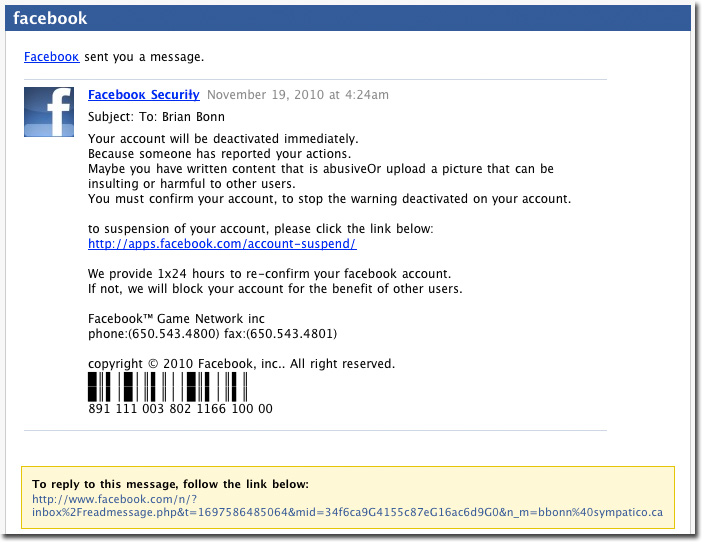
\includegraphics{facebook_phishing} \
 
\end{document}
